\chapter{Introduction}
\label{ch:intro}

\begin{comment}
Inductive Logic Programming (ILP) is a consolidated technique for mining first-order rules in knowledge
bases.
Nevertheless, it's inherently expensive and the hypothesis search space grows combinatorially with the knowledge base
size. 
This problem is even more dramatic when literals with constants are considered. Therefore, it usually requires
very aggressive pruning for making it feasible. 
Moreover, searching for rules with numerical intervals requires very expensive queries, and frequently do not bring
any significant confidence gain.
We propose a preprocessing step and an extension to ILP top-down algorithm, with the objective of efficiently learning
rules with interesting intervals for numerical attributes, i.e., rules which present a significant gain when restricting
a numerical attribute variable to a specific interval, combined with categorical constants.
In the preprocessing step, we build a lattice that expresses the correlations between a root numerical attribute and
multiple categorical relations and their constants, while in the refinement step of ILP, we query this lattice in order
to know whether it is interesting to search for numerical intervals, as well as obtain a list of refinement
suggestions ordered by a defined an interestingness measure.
This thesis discusses how to efficiently build the correlation lattice, how to incorporate it in the core ILP learning
algorithm, and compares different iterestingness measures. Also, we make experiments on large-scale linked data
sources in order to evaluate the proposed approach.


, and we extend
the ILP by adding to its refinement step a query to this lattice in order to obtain the interestingness of searching
for interesting intervals of a given numerical attribute variable, as well as a list of refinement suggestions ordered
by a defined an interestingness measure

consists of querying this lattice in
order to evaluate the potential of a given rule to have interesting intervals, as well as suggest a list of literals
which are interesting to add to the body of the rule.

. . This thesis
discusses how to efficiently build the lattice, how it's
incorporated in the core learning algorithm and evaluates different iterestingness measures.
\end{comment}


In the last years, the volume of semantic data available, in particular in RDF format, has dramatically
increased. Initiatives like the W3C Semantic Web and the Linked Open Data  have great contribution in such
development. The first provides a common standard that allows data to be shared and reused across different
applications and the latter provides linkages between different datasets that were not originally interconnected.
Moreover, advances in information extraction have also made a strong contribution, by crawling multiple non-structured
resources in the Web and extracting RDF facts.

Nevertheless, information extraction still has its limitations and many of its sources might contain contradictory
or uncertain information. Therefore, many of the extracted datasets suffer from incompleteness, noise and uncertainty.
The first one means that there are facts that are not existent in the dataset, the second one means that the dataset
might contain facts that are not true, and the latter one means that the truth of the facts is not certain. These
problems make it much more challenging to automatically learn rules from the data.

%Moreover, for noisy and incomplete knowledge bases, the automatic (i.e., unsupervised) selection of positive and
%negative training examples needed for learning new rules poses a major challenge to the adoption of these techniques.

In order to reduce such problems, one can apply a set of inference rules that describes the knowledge base domain.
With that, it is possible to resolve contradictions as well as strengthen or weaken their confidence values. It is
also possible to derive new facts that are originally not existent due to incompleteness. Such inference rules can
either represent consistency constraints (hard rules), or rules that hold for most but all cases in real world (soft
rules).

In this thesis, we consider only inference rules that can be represented as safe Datalog clauses. In a nutshell,
a Datalog clause is a logic program clause composed by a head predicates and a list of body predicates, each
predicate is a tuple with variables or constants as arguments. A Datalog clause is safe if all the variables present
in the head are also present in the body, moreover, negated predicates are allowed in the body as long as every
variable present in a negated predicate is also present in a non-negated predicate.

An example of safe Datalog rule, which states that married people usually live in the same place as their spouse,
could be written as follows:

\begin{center}
  $livesIn(X,Y)$ :- $marriedTo(X,Z),livesIn(Z,Y)$
\end{center}

If we have an incomplete knowledge base, which lacks information about where \emph{Michelle Obama} lives, but
contains the facts $marriedTo(michelleObama,barackObama)$ and $livesIn(barackObama,washingtonDC)$, we could then
apply the aforementioned rule to derive the fact $livesIn(michelleObama, washingtonDC)$. 


%http://people.csail.mit.edu/kersting/profile/PROFILE_ilp.html

Such rules are rarely known beforehand, but the data itself can be used to mine these rules using Inductive Logic
Programming (ILP). ILP is a well-established framework for inductively learning relational descriptions (in the form
of logic programs) from examples and background knowledge. Given a logical database of facts, an ILP system will
generate hypotheses in a pre-determined order and test them against the examples. However, in a large knowledge base,
ILP becomes too expensive as the search space grows combinatorially with the knowledge base size, and the larger the
number of examples, the more expensive it is to test each hypothesis.

Although it is very expensive to learn rules with constants, such kind of rules can be extremely interesting as they
can express particular characteristics of specific groups. For example, the rule $speaks(X,Y)$ :- $livesIn(X,Z)$ is not
very meaningful, it simply tells that people that live in anywhere will speak some language. Nevertheless, if we
consider setting constant values for $Y$ and $Z$, we can learn much more valuable rules such as
$speaks(X,english)$ :- $livesIn(X,australia)$ or $speaks(X,spanish)$ :- $livesIn(X,mexico)$.

The problem of that, is that for such an example, it would be necessary to test rules with all combinations of
countries and languages, which surely can lead to a very expensive process when applied on large databases. Given the
huge size of the search space and the great interestingness of rules with constants, it is appropriate to reduce the
search space by pruning constants or combinations of constants that do not have any correlation to the
hypothesis.

The literal $bornInMonth(X,april)$, for example, does not have any correlation  to $speaks(X,spanish )$ :-
$livesIn(X,mexico)$ or $speaks(X,english)$ :- $livesIn(X,australia)$. So if we ad such literal to the body of any of
theses clauses, it would most likely not cause any change to the confidence,  but crtanly a reduction in the support,
therefore it is not interesting to test these hypotheses with the addition of  such uncorelated literal.

%This will give as output a set of rules which should satisfy a minimum support and confidence.

\section{Motivation}

For numerical properties, it might be also relevant to search for interesting constants. Nevertheless, for very large
or infinite numerical domains such as the real numbers for example, setting a numerical constant as an individual
value will very likely have a single entity associated to it. In such a case, it would be equivalent to simply
specifying a constant for this given entity without the necessity of adding the numerical property

For example, it is extremely unlikely that a country has the exact same GDP or population as any other country. If we
have the following rule with the attribute $hasPopulation$, whose domain is the positive integer numbers
$\mathbb{N}^+$:

\begin{center}
 $speaks(X,portuguese)$ :- $livesIn(X,Z),hasPopulation(Z,193946886)$
\end{center}

As Brazil is the only country with a population of $193,946,886$ inhabitants, this same rule would be equivalent to:

\begin{center}
 $speaks(X,portuguese)$ :- $livesIn(X,brazil)$
\end{center}

Of course, if we have to choose between one of the two rules, the latter one would be preferred as it is shorter and
specifies the country in a clearer manner. Moreover, by setting numerical constants punctually, we would end up having a
huge number of different constants to test in the hypothesis and most of them would be most likely discarded because of
low support.

Therefore, it is interesting to discretize the numerical attribute's domain into categories, and
subsequently check if any of the buckets present different confidence in comparison to its correspondent numerical
constant-free rule (which we will call ``base-rule'').

For example if we test the hypothesis and we find support=40 and confidence=0.4:

\begin{center}
 $isMarriedTo(X,Y)$ :- $hasAge(X,Z)$ 
\end{center}

and then we split $Z$ into three buckets:

\begin{itemize}
 \item $ b_1: Z\in[0,20]$
 \item $ b_2: Z\in(20,40]$
 \item $ b_3: Z\in(40,\infty]$
\end{itemize}

we then generate three refined-rules by restricting the base-rule's domain from variable $Z$:

\begin{itemize}

 \item $isMarriedTo(X,Y)$ :- $hasAge(X,Z), z\in[0,20]$	
    \newline support=4, confidence=0.1
 \item $isMarriedTo(X,Y)$ :- $hasAge(X,Z), z\in(20,40]$	
    \newline support=20, confidence=0.5
 \item $isMarriedTo(X,Y)$ :- $hasAge(X,Z), z\in(40,\infty]$
    \newline support=16, confidence=0.8

\end{itemize}

for $b_2$ and $b_3$, the hypothesis has significant gain by specifying numerical constants. Adding a relation to the
body might produce totally different support and confidence distributions along the buckets. For example, if we add the
relation $hasChild(X,A)$, we could obtain other interesting rules:

Base-rule:
\begin{itemize}
 \item $sMarriedTo(X,Y)$ :- $hasAge(X,Z),hasChild(X,A)$	
    \newline support=32, confidence=0.76
\end{itemize}

Refined-rules:
\begin{itemize}
 \item $isMarriedTo(X,Y)$ :- $hasAge(X,Z),hasChild(x,a), Z\in[0,20]$	
    \newline support=1, confidence=0.5
 \item $isMarriedTo(X,Y)$ :- $hasAge(X,Z),hasChild(x,a), Z\in(20,40]$	
    \newline support=15, confidence=0.75
 \item $isMarriedTo(X,Y)$ :- $hasAge(X,Z),hasChild(x,a), Z\in(40,\infty]$	
    \newline support=16, confidence=0.8
\end{itemize}

\begin{figure}
\label{fig:addingHasChildExample}

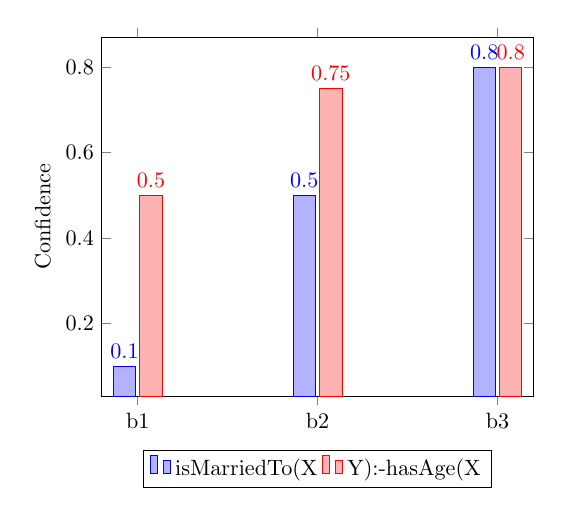
\begin{tikzpicture}[scale=0.8]
\begin{axis}[
    ybar,
    enlargelimits=0.10,
    legend style={at={(0.5,-0.15)},
      anchor=north,legend columns=-1},
    ylabel={Confidence},
    symbolic x coords={b1,b2,b3},
    xtick=data,
    nodes near coords,
    nodes near coords align={vertical},
    ]
\addplot coordinates {(b1,0.1) (b2,0.5) (b3,0.8)};
\addplot coordinates {(b1,0.5) (b2,0.75) (b3,0.8)};
\legend{isMarriedTo(X,Y):-hasAge(X,Z) , isMarriedTo(X,Y):-hasAge(X,Z)hasChild(X,A)}
\end{axis}
\end{tikzpicture}
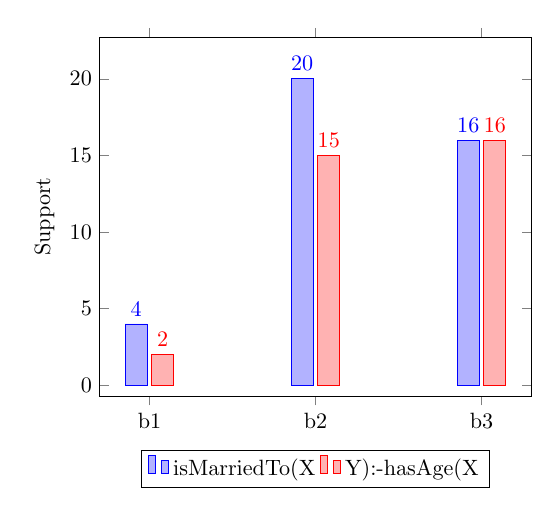
\begin{tikzpicture}[scale=0.8]
\begin{axis}[
    ybar,
    enlargelimits=0.15,
    legend style={at={(0.5,-0.15)},
      anchor=north,legend columns=-1},
    ylabel={Support},
    symbolic x coords={b1,b2,b3},
    xtick=data,
    nodes near coords,
    nodes near coords align={vertical},
    ]
\addplot coordinates {(b1,4) (b2,20) (b3,16)};
\addplot coordinates {(b1, 2) (b2,15) (b3,16)};
\legend{isMarriedTo(X,Y):-hasAge(X,Z), isMarriedTo(X,Y):-hasAge(X,Z)hasChild(X,A)}
\end{axis}
\end{tikzpicture}
\end{figure}

Adding a given predicate to the rule might not bring any gain or even loss in confidence to the base-rule, but when
bucketing per age, present a different confidence and support distribution and might even produce gain in confidence for
some specific buckets.

Nevertheless, adding a predicate with no correlation to the rule might not generate any gain. Thus, it's necessary to
carefully choose the relations and eventual constants and discard the ones with no correlation to the rule.  

\section{Contributions}
In this thesis, we propose a pre-processing step to build a graph we call correlation lattice for each numerical
property we want to for interesting intervals. In each graph, that has a numerical property as its root, we first
query the examples distribution on the numerical attribute, and build a histogram by discretizing them into $k$
buckets. Subsequently, we  pick a set of $c$ categorical properties that can be joined with the root, extract the
frequencies histogram and analyze how the distribution of sub-population created by joining them with the root is
affected. Afterwards, we try to combine the categories and check whether they still produce interesting sub-populations
creating a lattice, like in frequent set mining apriori algorithm.

We compare the distributions obtained from the frequencies histograms using information theoretical measures,
such as Kullback-Leibler divergence, as well as independence checks, such as Pearson's Chi-squared, in order to
measure the interestingness of adding literals to clauses.

Moreover, we discuss the pruning opportunities and also evaluate different heuristics and interestingness measures and
their efficiency in finding rules with numerical intervals. 

\begin{comment}
In a clause containing a numerical attribute in the body, we can obtain a support and confidence as well as support
value for each of the buckets. Therewith, we can search the most interesting intervals that satisfies the support and
confidence thresholds
\end{comment}

With information about different example distributions contained in the generated lattice, once we add one of the root
properties during the core ILP algorithm, we can try to predict whether the rule has interesting intervals for the
given numerical attribute, and prevent unnecessary expensive queries to be fired. Furthermore, for a given clause, we
can also suggest the most interesting literals to be added to the body of the clause.

In summary, we present in this thesis three main contributions:

\begin{itemize}
 \item A measure of the interestingness of searching for a specific interval for a rule's numerical attribute
variable.
 \item The correlation lattice and its pruning methods.
 \item Experiments on Linked Open Data datasets.
\end{itemize}


\section{Outline}

\begin{comment}
 The remainder of this thesis is structured as follows. In
Chapter~\ref{ch:technical_background}, we provide technical background on
MapReduce and BigTable. In Chapter~\ref{ch:related_work}, we present a
summary of previous work in the areas of duplicate and near-duplicate detection,
information retrieval on web archives, and MapReduce applications in graph
processing. Following that, we state our problem and describe solutions in
Chapter~\ref{ch:redundancy_control}. In Chapter~\ref{ch:mapreduce_impl}, we
describe an implementation of our solution using the MapReduce framework. In
Chapter~\ref{ch:experiments}, we present our experimental results. We conclude
this thesis and outline directions of future research in Chapter~\ref{ch:future_work}.
\end{comment}
